% $Id: getdp.tex,v 1.1 2001-06-11 07:50:49 geuzaine Exp $

% ---------------------------------------------------------------------------

\chapter{}

\begin{slide}

\slidepagestyle{reduced}

\begin{center}
\bigtitle{A general software environment for the treatment of discrete problems}\\
\bigtitle{(GetDP)}\\
\bigskip\bigskip
\medtitle{Patrick Dular and Christophe Geuzaine}\\
\bigskip
\medtitle{Department of Electrical Engineering}\\
\medtitle{Montefiore Institute B28, Sart Tilman Campus}\\
\medtitle{University of Li�ge}\\
\medtitle{B-4000 Li�ge (BELGIUM)}
\end{center}

\end{slide}

% ---------------------------------------------------------------------------
\part{GetDP}
% ---------------------------------------------------------------------------

\chapter{An environment open to various couplings}

\begin{slide}

Any coupling between 
\begin{slideitemize}
\item \emph{Physical} problems (electromagnetic, thermal, mechanical, ...)
\item \emph{Numerical} methods (finite element methods, integral methods, ...)
\item \emph{Geometries} (1D, 2D, 2D axi, 3D)
\item \emph{Time} states (static, harmonic, transient)
\end{slideitemize}

How?
\begin{slideitemize}
\item Clear \emph{mathematical} definitions/structure
\item Directly transcribed into 10 interdependent \emph{objects}
\end{slideitemize}

\end{slide}

% ---------------------------------------------------------------------------

\chapter{Definition of discrete problems}

\begin{slide}

\begin{slideitemize}
\item Copy of formal mathematical expression of problems 
\item ASCII \emph{Text} file (``\code{.pro} file'')
\end{slideitemize}

\begin{center}
\scalebox{0.54}{\begin{picture}(0,0)%
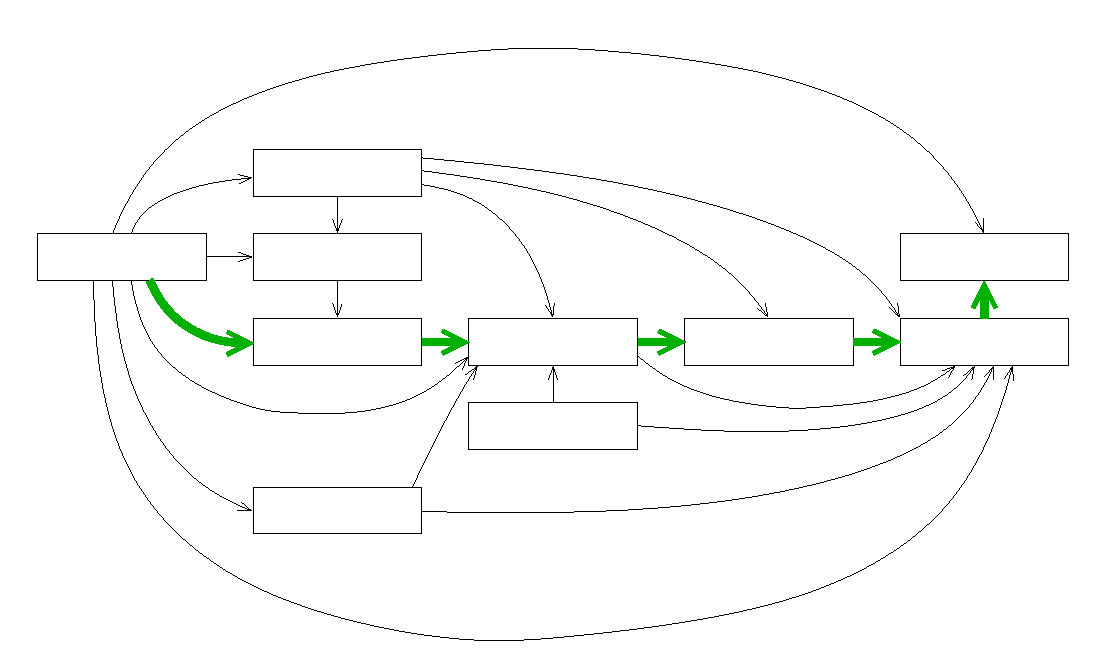
\includegraphics{getdp-struct}%
\end{picture}%
\setlength{\unitlength}{3947sp}%
%
\begingroup\makeatletter\ifx\SetFigFont\undefined%
\gdef\SetFigFont#1#2#3#4#5{%
  \reset@font\fontsize{#1}{#2pt}%
  \fontfamily{#3}\fontseries{#4}\fontshape{#5}%
  \selectfont}%
\fi\endgroup%
\begin{picture}(8552,4992)(300,-6402)
\put(1126,-3361){\makebox(0,0)[b]{\smash{\SetFigFont{10}{12.0}{\rmdefault}{\mddefault}{\updefault}{\color[rgb]{0,0,0}\code{Group}}%
}}}
\put(2851,-2686){\makebox(0,0)[b]{\smash{\SetFigFont{10}{12.0}{\rmdefault}{\mddefault}{\updefault}{\color[rgb]{0,0,0}\code{Function}}%
}}}
\put(2851,-3361){\makebox(0,0)[b]{\smash{\SetFigFont{10}{12.0}{\rmdefault}{\mddefault}{\updefault}{\color[rgb]{0,0,0}\code{Constraint}}%
}}}
\put(2851,-4036){\makebox(0,0)[b]{\smash{\SetFigFont{10}{12.0}{\rmdefault}{\mddefault}{\updefault}{\color[rgb]{0,0,0}\code{FunctionSpace}}%
}}}
\put(2851,-5386){\makebox(0,0)[b]{\smash{\SetFigFont{10}{12.0}{\rmdefault}{\mddefault}{\updefault}{\color[rgb]{0,0,0}\code{Jacobian}}%
}}}
\put(4576,-4711){\makebox(0,0)[b]{\smash{\SetFigFont{10}{12.0}{\rmdefault}{\mddefault}{\updefault}{\color[rgb]{0,0,0}\code{Integration}}%
}}}
\put(4576,-4036){\makebox(0,0)[b]{\smash{\SetFigFont{10}{12.0}{\rmdefault}{\mddefault}{\updefault}{\color[rgb]{0,0,0}\code{Formulation}}%
}}}
\put(6301,-4036){\makebox(0,0)[b]{\smash{\SetFigFont{10}{12.0}{\rmdefault}{\mddefault}{\updefault}{\color[rgb]{0,0,0}\code{Resolution}}%
}}}
\put(8026,-3361){\makebox(0,0)[b]{\smash{\SetFigFont{10}{12.0}{\rmdefault}{\mddefault}{\updefault}{\color[rgb]{0,0,0}\code{PostOperation}}%
}}}
\put(8026,-4036){\makebox(0,0)[b]{\smash{\SetFigFont{10}{12.0}{\rmdefault}{\mddefault}{\updefault}{\color[rgb]{0,0,0}\code{PostProcessing}}%
}}}
\end{picture}
}
\end{center}

\end{slide}

\begin{slide}

\begin{center}
Particular data of a problem\\
\medskip
\scalebox{0.54}{\begin{picture}(0,0)%
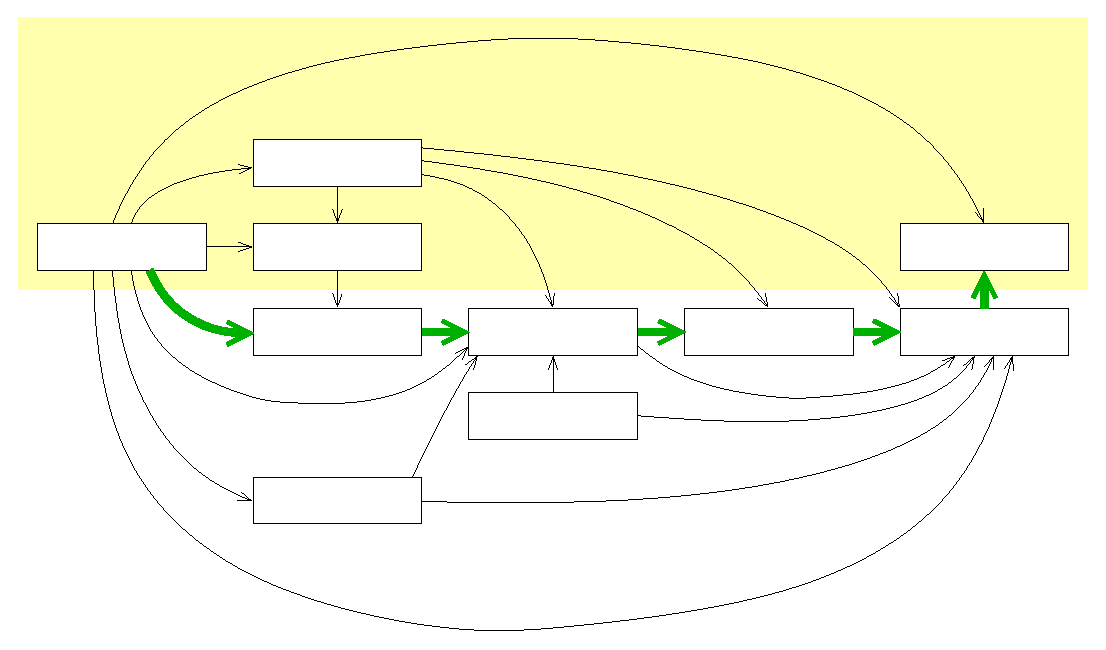
\includegraphics{getdp-struct-box}%
\end{picture}%
\setlength{\unitlength}{3947sp}%
%
\begingroup\makeatletter\ifx\SetFigFont\undefined%
\gdef\SetFigFont#1#2#3#4#5{%
  \reset@font\fontsize{#1}{#2pt}%
  \fontfamily{#3}\fontseries{#4}\fontshape{#5}%
  \selectfont}%
\fi\endgroup%
\begin{picture}(8552,4917)(300,-6402)
\put(1126,-3361){\makebox(0,0)[b]{\smash{\SetFigFont{10}{12.0}{\rmdefault}{\mddefault}{\updefault}{\color[rgb]{0,0,0}\code{Group}}%
}}}
\put(2851,-2686){\makebox(0,0)[b]{\smash{\SetFigFont{10}{12.0}{\rmdefault}{\mddefault}{\updefault}{\color[rgb]{0,0,0}\code{Function}}%
}}}
\put(2851,-3361){\makebox(0,0)[b]{\smash{\SetFigFont{10}{12.0}{\rmdefault}{\mddefault}{\updefault}{\color[rgb]{0,0,0}\code{Constraint}}%
}}}
\put(2851,-4036){\makebox(0,0)[b]{\smash{\SetFigFont{10}{12.0}{\rmdefault}{\mddefault}{\updefault}{\color[rgb]{0,0,0}\code{FunctionSpace}}%
}}}
\put(2851,-5386){\makebox(0,0)[b]{\smash{\SetFigFont{10}{12.0}{\rmdefault}{\mddefault}{\updefault}{\color[rgb]{0,0,0}\code{Jacobian}}%
}}}
\put(4576,-4711){\makebox(0,0)[b]{\smash{\SetFigFont{10}{12.0}{\rmdefault}{\mddefault}{\updefault}{\color[rgb]{0,0,0}\code{Integration}}%
}}}
\put(4576,-4036){\makebox(0,0)[b]{\smash{\SetFigFont{10}{12.0}{\rmdefault}{\mddefault}{\updefault}{\color[rgb]{0,0,0}\code{Formulation}}%
}}}
\put(6301,-4036){\makebox(0,0)[b]{\smash{\SetFigFont{10}{12.0}{\rmdefault}{\mddefault}{\updefault}{\color[rgb]{0,0,0}\code{Resolution}}%
}}}
\put(8026,-3361){\makebox(0,0)[b]{\smash{\SetFigFont{10}{12.0}{\rmdefault}{\mddefault}{\updefault}{\color[rgb]{0,0,0}\code{PostOperation}}%
}}}
\put(8026,-4036){\makebox(0,0)[b]{\smash{\SetFigFont{10}{12.0}{\rmdefault}{\mddefault}{\updefault}{\color[rgb]{0,0,0}\code{PostProcessing}}%
}}}
\end{picture}
}\\
\medskip
Method of resolution (``black box'')
\end{center}

\end{slide}

% ---------------------------------------------------------------------------

\background{7\semcm}{4.2\semcm}{\scalebox{0.3}{\begin{picture}(0,0)%
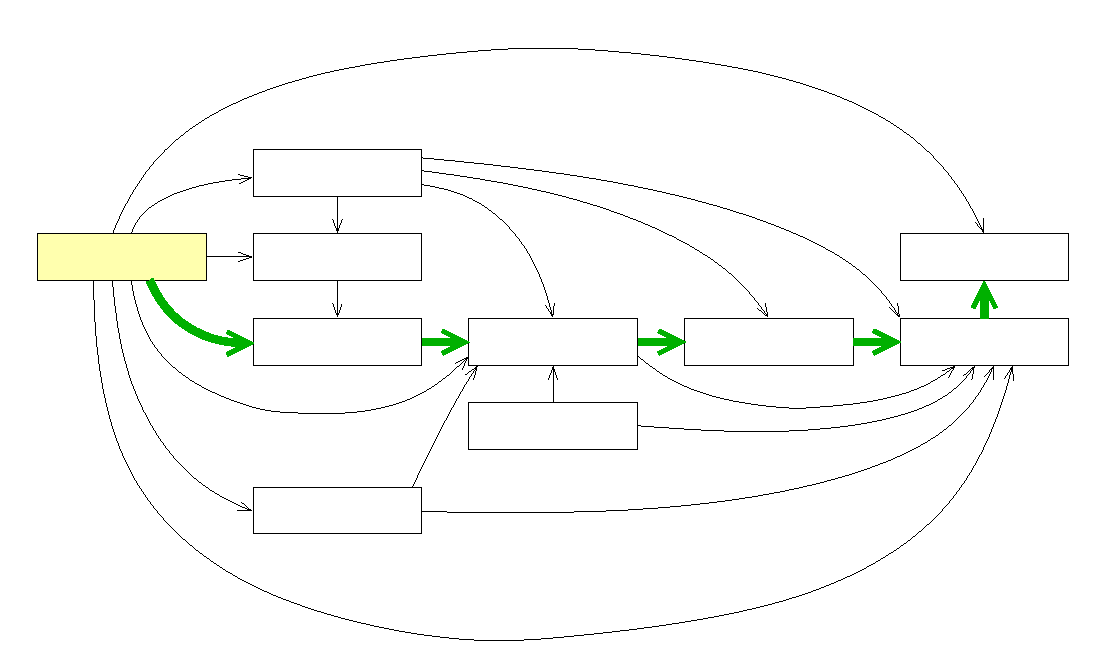
\includegraphics{getdp-struct-group}%
\end{picture}%
\setlength{\unitlength}{3947sp}%
%
\begingroup\makeatletter\ifx\SetFigFont\undefined%
\gdef\SetFigFont#1#2#3#4#5{%
  \reset@font\fontsize{#1}{#2pt}%
  \fontfamily{#3}\fontseries{#4}\fontshape{#5}%
  \selectfont}%
\fi\endgroup%
\begin{picture}(8274,4765)(439,-6402)
\put(1126,-3361){\makebox(0,0)[b]{\smash{\SetFigFont{10}{12.0}{\rmdefault}{\mddefault}{\updefault}{\color[rgb]{0,0,0}\code{Group}}%
}}}
\put(2851,-2686){\makebox(0,0)[b]{\smash{\SetFigFont{10}{12.0}{\rmdefault}{\mddefault}{\updefault}{\color[rgb]{0,0,0}\code{Function}}%
}}}
\put(2851,-3361){\makebox(0,0)[b]{\smash{\SetFigFont{10}{12.0}{\rmdefault}{\mddefault}{\updefault}{\color[rgb]{0,0,0}\code{Constraint}}%
}}}
\put(2851,-4036){\makebox(0,0)[b]{\smash{\SetFigFont{10}{12.0}{\rmdefault}{\mddefault}{\updefault}{\color[rgb]{0,0,0}\code{FunctionSpace}}%
}}}
\put(2851,-5386){\makebox(0,0)[b]{\smash{\SetFigFont{10}{12.0}{\rmdefault}{\mddefault}{\updefault}{\color[rgb]{0,0,0}\code{Jacobian}}%
}}}
\put(4576,-4711){\makebox(0,0)[b]{\smash{\SetFigFont{10}{12.0}{\rmdefault}{\mddefault}{\updefault}{\color[rgb]{0,0,0}\code{Integration}}%
}}}
\put(4576,-4036){\makebox(0,0)[b]{\smash{\SetFigFont{10}{12.0}{\rmdefault}{\mddefault}{\updefault}{\color[rgb]{0,0,0}\code{Formulation}}%
}}}
\put(6301,-4036){\makebox(0,0)[b]{\smash{\SetFigFont{10}{12.0}{\rmdefault}{\mddefault}{\updefault}{\color[rgb]{0,0,0}\code{Resolution}}%
}}}
\put(8026,-3361){\makebox(0,0)[b]{\smash{\SetFigFont{10}{12.0}{\rmdefault}{\mddefault}{\updefault}{\color[rgb]{0,0,0}\code{PostOperation}}%
}}}
\put(8026,-4036){\makebox(0,0)[b]{\smash{\SetFigFont{10}{12.0}{\rmdefault}{\mddefault}{\updefault}{\color[rgb]{0,0,0}\code{PostProcessing}}%
}}}
\end{picture}
}}

\chapter{\code{Group}: defining topological entities}

\begin{slide}

\mybox{colbox}{11\semcm}{
  \begin{slideitemize}
  \item Regions
  \item Functions on Regions (nodes, edges, edges of tree, ...)
  \end{slideitemize}
}

Example:

\begin{syntax}
Air = Region[1]; Core = Region[2];
    = ;
\end{syntax}



\end{slide}

% ---------------------------------------------------------------------------

\background{7\semcm}{4.2\semcm}{\scalebox{0.3}{\begin{picture}(0,0)%
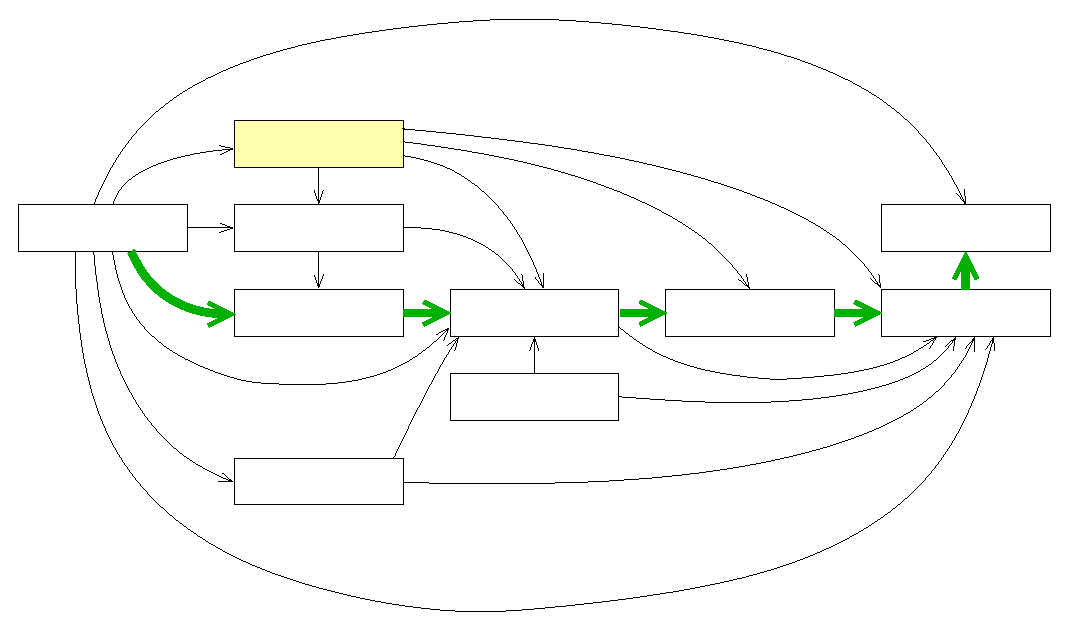
\includegraphics{getdp-struct-function}%
\end{picture}%
\setlength{\unitlength}{3947sp}%
%
\begingroup\makeatletter\ifx\SetFigFont\undefined%
\gdef\SetFigFont#1#2#3#4#5{%
  \reset@font\fontsize{#1}{#2pt}%
  \fontfamily{#3}\fontseries{#4}\fontshape{#5}%
  \selectfont}%
\fi\endgroup%
\begin{picture}(8274,4765)(439,-6402)
\put(1126,-3361){\makebox(0,0)[b]{\smash{\SetFigFont{10}{12.0}{\rmdefault}{\mddefault}{\updefault}{\color[rgb]{0,0,0}\code{Group}}%
}}}
\put(2851,-2686){\makebox(0,0)[b]{\smash{\SetFigFont{10}{12.0}{\rmdefault}{\mddefault}{\updefault}{\color[rgb]{0,0,0}\code{Function}}%
}}}
\put(2851,-3361){\makebox(0,0)[b]{\smash{\SetFigFont{10}{12.0}{\rmdefault}{\mddefault}{\updefault}{\color[rgb]{0,0,0}\code{Constraint}}%
}}}
\put(2851,-4036){\makebox(0,0)[b]{\smash{\SetFigFont{10}{12.0}{\rmdefault}{\mddefault}{\updefault}{\color[rgb]{0,0,0}\code{FunctionSpace}}%
}}}
\put(2851,-5386){\makebox(0,0)[b]{\smash{\SetFigFont{10}{12.0}{\rmdefault}{\mddefault}{\updefault}{\color[rgb]{0,0,0}\code{Jacobian}}%
}}}
\put(4576,-4711){\makebox(0,0)[b]{\smash{\SetFigFont{10}{12.0}{\rmdefault}{\mddefault}{\updefault}{\color[rgb]{0,0,0}\code{Integration}}%
}}}
\put(4576,-4036){\makebox(0,0)[b]{\smash{\SetFigFont{10}{12.0}{\rmdefault}{\mddefault}{\updefault}{\color[rgb]{0,0,0}\code{Formulation}}%
}}}
\put(6301,-4036){\makebox(0,0)[b]{\smash{\SetFigFont{10}{12.0}{\rmdefault}{\mddefault}{\updefault}{\color[rgb]{0,0,0}\code{Resolution}}%
}}}
\put(8026,-3361){\makebox(0,0)[b]{\smash{\SetFigFont{10}{12.0}{\rmdefault}{\mddefault}{\updefault}{\color[rgb]{0,0,0}\code{PostOperation}}%
}}}
\put(8026,-4036){\makebox(0,0)[b]{\smash{\SetFigFont{10}{12.0}{\rmdefault}{\mddefault}{\updefault}{\color[rgb]{0,0,0}\code{PostProcessing}}%
}}}
\end{picture}
}}

\chapter{\code{Function}: defining expressions}

\begin{slide}

\mybox{colbox}{11\semcm}{
  \begin{slideitemize}
  \item Physical characteristics
  \item Time functions
  \item Various other functions (natural contraints, ...)
  \end{slideitemize}
}

Example:


\end{slide}

% ---------------------------------------------------------------------------

\background{7\semcm}{4.2\semcm}{\scalebox{0.3}{\begin{picture}(0,0)%
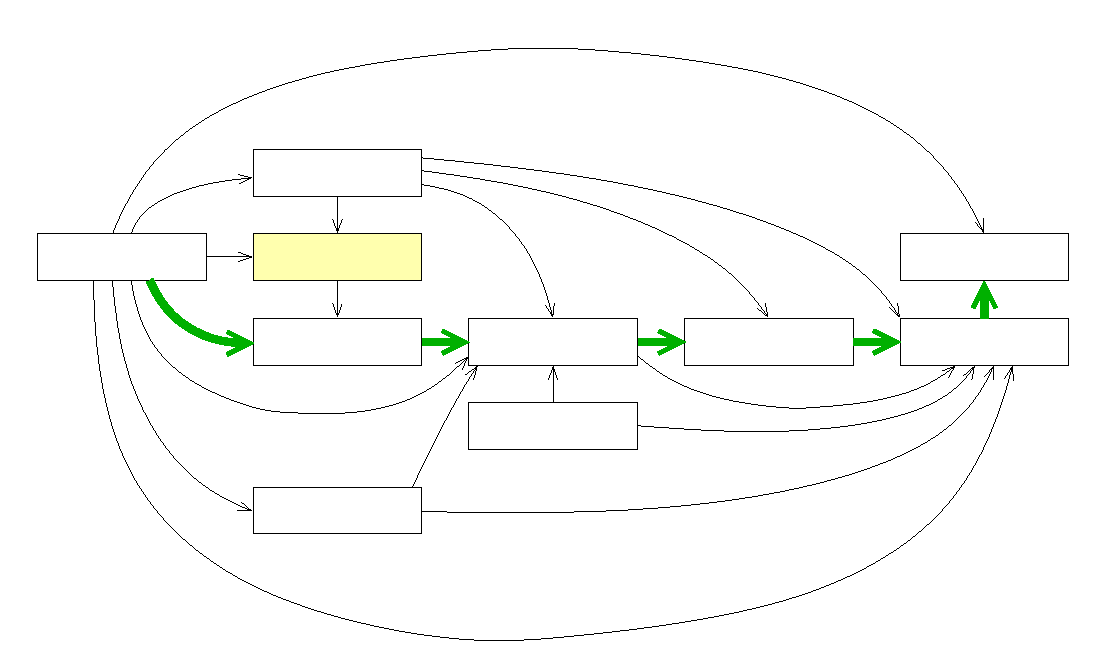
\includegraphics{getdp-struct-constraint}%
\end{picture}%
\setlength{\unitlength}{3947sp}%
%
\begingroup\makeatletter\ifx\SetFigFont\undefined%
\gdef\SetFigFont#1#2#3#4#5{%
  \reset@font\fontsize{#1}{#2pt}%
  \fontfamily{#3}\fontseries{#4}\fontshape{#5}%
  \selectfont}%
\fi\endgroup%
\begin{picture}(8274,4765)(439,-6402)
\put(1126,-3361){\makebox(0,0)[b]{\smash{\SetFigFont{10}{12.0}{\rmdefault}{\mddefault}{\updefault}{\color[rgb]{0,0,0}\code{Group}}%
}}}
\put(2851,-2686){\makebox(0,0)[b]{\smash{\SetFigFont{10}{12.0}{\rmdefault}{\mddefault}{\updefault}{\color[rgb]{0,0,0}\code{Function}}%
}}}
\put(2851,-3361){\makebox(0,0)[b]{\smash{\SetFigFont{10}{12.0}{\rmdefault}{\mddefault}{\updefault}{\color[rgb]{0,0,0}\code{Constraint}}%
}}}
\put(2851,-4036){\makebox(0,0)[b]{\smash{\SetFigFont{10}{12.0}{\rmdefault}{\mddefault}{\updefault}{\color[rgb]{0,0,0}\code{FunctionSpace}}%
}}}
\put(2851,-5386){\makebox(0,0)[b]{\smash{\SetFigFont{10}{12.0}{\rmdefault}{\mddefault}{\updefault}{\color[rgb]{0,0,0}\code{Jacobian}}%
}}}
\put(4576,-4711){\makebox(0,0)[b]{\smash{\SetFigFont{10}{12.0}{\rmdefault}{\mddefault}{\updefault}{\color[rgb]{0,0,0}\code{Integration}}%
}}}
\put(4576,-4036){\makebox(0,0)[b]{\smash{\SetFigFont{10}{12.0}{\rmdefault}{\mddefault}{\updefault}{\color[rgb]{0,0,0}\code{Formulation}}%
}}}
\put(6301,-4036){\makebox(0,0)[b]{\smash{\SetFigFont{10}{12.0}{\rmdefault}{\mddefault}{\updefault}{\color[rgb]{0,0,0}\code{Resolution}}%
}}}
\put(8026,-3361){\makebox(0,0)[b]{\smash{\SetFigFont{10}{12.0}{\rmdefault}{\mddefault}{\updefault}{\color[rgb]{0,0,0}\code{PostOperation}}%
}}}
\put(8026,-4036){\makebox(0,0)[b]{\smash{\SetFigFont{10}{12.0}{\rmdefault}{\mddefault}{\updefault}{\color[rgb]{0,0,0}\code{PostProcessing}}%
}}}
\end{picture}
}}

\chapter{\code{Constraint}: specifying constraints}

\begin{slide}

\mybox{colbox}{11\semcm}{
  \begin{slideitemize}
  \item Boundary conditions (classical, connection)
  \item Initial conditions
  \item Topology of circuits with lumped elements
  \item Other constraints (on local and global quantities)
  \end{slideitemize}
}

Example:


\end{slide}

% ---------------------------------------------------------------------------

\background{7\semcm}{4.2\semcm}{\scalebox{0.3}{\begin{picture}(0,0)%
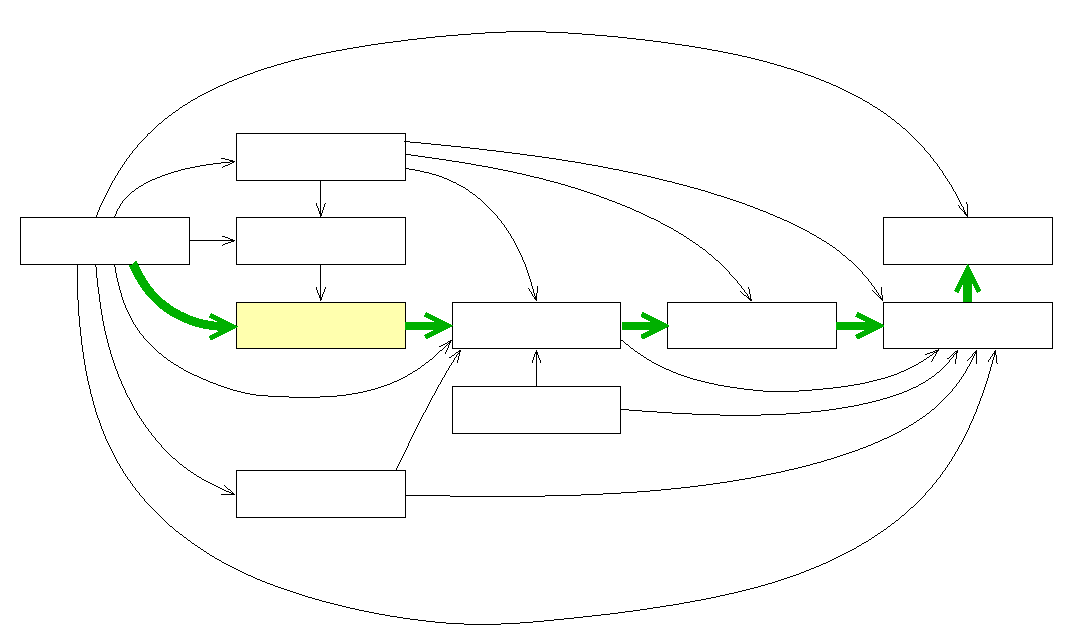
\includegraphics{getdp-struct-functionspace}%
\end{picture}%
\setlength{\unitlength}{3947sp}%
%
\begingroup\makeatletter\ifx\SetFigFont\undefined%
\gdef\SetFigFont#1#2#3#4#5{%
  \reset@font\fontsize{#1}{#2pt}%
  \fontfamily{#3}\fontseries{#4}\fontshape{#5}%
  \selectfont}%
\fi\endgroup%
\begin{picture}(8552,4992)(300,-6402)
\put(1126,-3361){\makebox(0,0)[b]{\smash{\SetFigFont{10}{12.0}{\rmdefault}{\mddefault}{\updefault}{\color[rgb]{0,0,0}\code{Group}}%
}}}
\put(2851,-2686){\makebox(0,0)[b]{\smash{\SetFigFont{10}{12.0}{\rmdefault}{\mddefault}{\updefault}{\color[rgb]{0,0,0}\code{Function}}%
}}}
\put(2851,-3361){\makebox(0,0)[b]{\smash{\SetFigFont{10}{12.0}{\rmdefault}{\mddefault}{\updefault}{\color[rgb]{0,0,0}\code{Constraint}}%
}}}
\put(2851,-4036){\makebox(0,0)[b]{\smash{\SetFigFont{10}{12.0}{\rmdefault}{\mddefault}{\updefault}{\color[rgb]{0,0,0}\code{FunctionSpace}}%
}}}
\put(2851,-5386){\makebox(0,0)[b]{\smash{\SetFigFont{10}{12.0}{\rmdefault}{\mddefault}{\updefault}{\color[rgb]{0,0,0}\code{Jacobian}}%
}}}
\put(4576,-4711){\makebox(0,0)[b]{\smash{\SetFigFont{10}{12.0}{\rmdefault}{\mddefault}{\updefault}{\color[rgb]{0,0,0}\code{Integration}}%
}}}
\put(4576,-4036){\makebox(0,0)[b]{\smash{\SetFigFont{10}{12.0}{\rmdefault}{\mddefault}{\updefault}{\color[rgb]{0,0,0}\code{Formulation}}%
}}}
\put(6301,-4036){\makebox(0,0)[b]{\smash{\SetFigFont{10}{12.0}{\rmdefault}{\mddefault}{\updefault}{\color[rgb]{0,0,0}\code{Resolution}}%
}}}
\put(8026,-3361){\makebox(0,0)[b]{\smash{\SetFigFont{10}{12.0}{\rmdefault}{\mddefault}{\updefault}{\color[rgb]{0,0,0}\code{PostOperation}}%
}}}
\put(8026,-4036){\makebox(0,0)[b]{\smash{\SetFigFont{10}{12.0}{\rmdefault}{\mddefault}{\updefault}{\color[rgb]{0,0,0}\code{PostProcessing}}%
}}}
\end{picture}
}}

\chapter{\code{FunctionSpace}: building function spaces}

\begin{slide}



Example:


\end{slide}

% ---------------------------------------------------------------------------

\background{7\semcm}{4.2\semcm}{\scalebox{0.3}{\begin{picture}(0,0)%
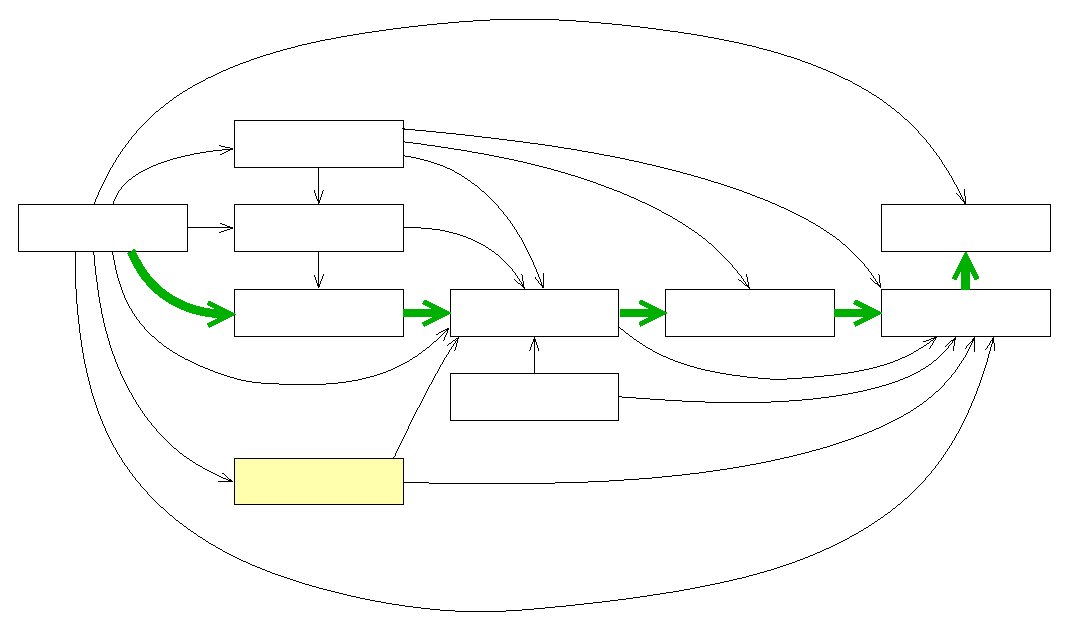
\includegraphics{getdp-struct-jacobian}%
\end{picture}%
\setlength{\unitlength}{3947sp}%
%
\begingroup\makeatletter\ifx\SetFigFont\undefined%
\gdef\SetFigFont#1#2#3#4#5{%
  \reset@font\fontsize{#1}{#2pt}%
  \fontfamily{#3}\fontseries{#4}\fontshape{#5}%
  \selectfont}%
\fi\endgroup%
\begin{picture}(8274,4765)(439,-6402)
\put(1126,-3361){\makebox(0,0)[b]{\smash{\SetFigFont{10}{12.0}{\rmdefault}{\mddefault}{\updefault}{\color[rgb]{0,0,0}\code{Group}}%
}}}
\put(2851,-2686){\makebox(0,0)[b]{\smash{\SetFigFont{10}{12.0}{\rmdefault}{\mddefault}{\updefault}{\color[rgb]{0,0,0}\code{Function}}%
}}}
\put(2851,-3361){\makebox(0,0)[b]{\smash{\SetFigFont{10}{12.0}{\rmdefault}{\mddefault}{\updefault}{\color[rgb]{0,0,0}\code{Constraint}}%
}}}
\put(2851,-4036){\makebox(0,0)[b]{\smash{\SetFigFont{10}{12.0}{\rmdefault}{\mddefault}{\updefault}{\color[rgb]{0,0,0}\code{FunctionSpace}}%
}}}
\put(2851,-5386){\makebox(0,0)[b]{\smash{\SetFigFont{10}{12.0}{\rmdefault}{\mddefault}{\updefault}{\color[rgb]{0,0,0}\code{Jacobian}}%
}}}
\put(4576,-4711){\makebox(0,0)[b]{\smash{\SetFigFont{10}{12.0}{\rmdefault}{\mddefault}{\updefault}{\color[rgb]{0,0,0}\code{Integration}}%
}}}
\put(4576,-4036){\makebox(0,0)[b]{\smash{\SetFigFont{10}{12.0}{\rmdefault}{\mddefault}{\updefault}{\color[rgb]{0,0,0}\code{Formulation}}%
}}}
\put(6301,-4036){\makebox(0,0)[b]{\smash{\SetFigFont{10}{12.0}{\rmdefault}{\mddefault}{\updefault}{\color[rgb]{0,0,0}\code{Resolution}}%
}}}
\put(8026,-3361){\makebox(0,0)[b]{\smash{\SetFigFont{10}{12.0}{\rmdefault}{\mddefault}{\updefault}{\color[rgb]{0,0,0}\code{PostOperation}}%
}}}
\put(8026,-4036){\makebox(0,0)[b]{\smash{\SetFigFont{10}{12.0}{\rmdefault}{\mddefault}{\updefault}{\color[rgb]{0,0,0}\code{PostProcessing}}%
}}}
\end{picture}
}}

\chapter{\code{Jacobian}: defining jacobian methods}

\begin{slide}


Example:


\end{slide}

% ---------------------------------------------------------------------------

\background{7\semcm}{4.2\semcm}{\scalebox{0.3}{\begin{picture}(0,0)%
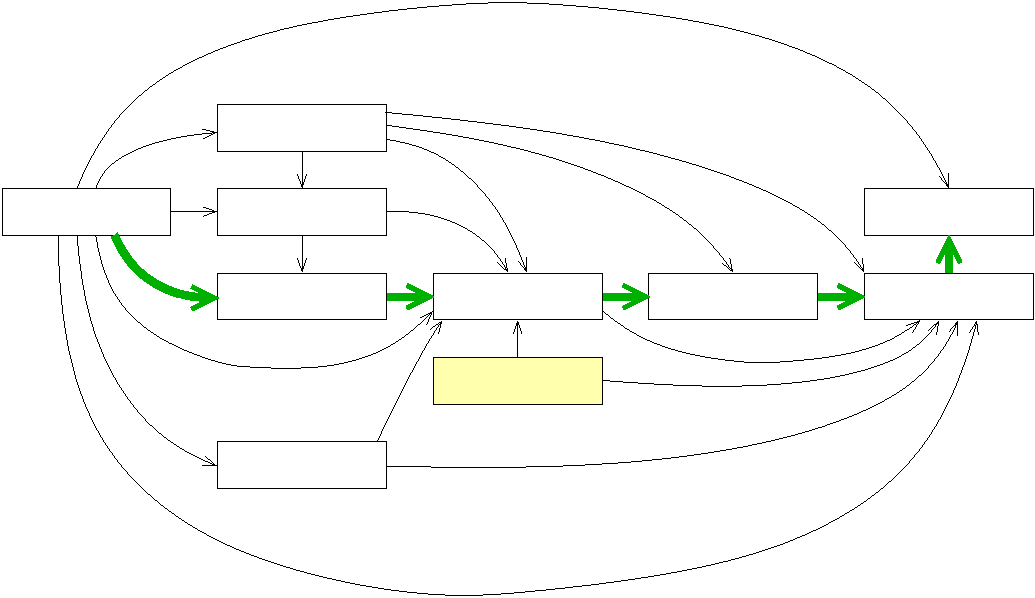
\includegraphics{getdp-struct-integration}%
\end{picture}%
\setlength{\unitlength}{3947sp}%
%
\begingroup\makeatletter\ifx\SetFigFont\undefined%
\gdef\SetFigFont#1#2#3#4#5{%
  \reset@font\fontsize{#1}{#2pt}%
  \fontfamily{#3}\fontseries{#4}\fontshape{#5}%
  \selectfont}%
\fi\endgroup%
\begin{picture}(8552,4992)(300,-6402)
\put(1126,-3361){\makebox(0,0)[b]{\smash{\SetFigFont{10}{12.0}{\rmdefault}{\mddefault}{\updefault}{\color[rgb]{0,0,0}\code{Group}}%
}}}
\put(2851,-2686){\makebox(0,0)[b]{\smash{\SetFigFont{10}{12.0}{\rmdefault}{\mddefault}{\updefault}{\color[rgb]{0,0,0}\code{Function}}%
}}}
\put(2851,-3361){\makebox(0,0)[b]{\smash{\SetFigFont{10}{12.0}{\rmdefault}{\mddefault}{\updefault}{\color[rgb]{0,0,0}\code{Constraint}}%
}}}
\put(2851,-4036){\makebox(0,0)[b]{\smash{\SetFigFont{10}{12.0}{\rmdefault}{\mddefault}{\updefault}{\color[rgb]{0,0,0}\code{FunctionSpace}}%
}}}
\put(2851,-5386){\makebox(0,0)[b]{\smash{\SetFigFont{10}{12.0}{\rmdefault}{\mddefault}{\updefault}{\color[rgb]{0,0,0}\code{Jacobian}}%
}}}
\put(4576,-4711){\makebox(0,0)[b]{\smash{\SetFigFont{10}{12.0}{\rmdefault}{\mddefault}{\updefault}{\color[rgb]{0,0,0}\code{Integration}}%
}}}
\put(4576,-4036){\makebox(0,0)[b]{\smash{\SetFigFont{10}{12.0}{\rmdefault}{\mddefault}{\updefault}{\color[rgb]{0,0,0}\code{Formulation}}%
}}}
\put(6301,-4036){\makebox(0,0)[b]{\smash{\SetFigFont{10}{12.0}{\rmdefault}{\mddefault}{\updefault}{\color[rgb]{0,0,0}\code{Resolution}}%
}}}
\put(8026,-3361){\makebox(0,0)[b]{\smash{\SetFigFont{10}{12.0}{\rmdefault}{\mddefault}{\updefault}{\color[rgb]{0,0,0}\code{PostOperation}}%
}}}
\put(8026,-4036){\makebox(0,0)[b]{\smash{\SetFigFont{10}{12.0}{\rmdefault}{\mddefault}{\updefault}{\color[rgb]{0,0,0}\code{PostProcessing}}%
}}}
\end{picture}
}}

\chapter{\code{Integration}: defining integration methods}

\begin{slide}



Example:


\end{slide}

% ---------------------------------------------------------------------------

\background{7\semcm}{4.2\semcm}{\scalebox{0.3}{\begin{picture}(0,0)%
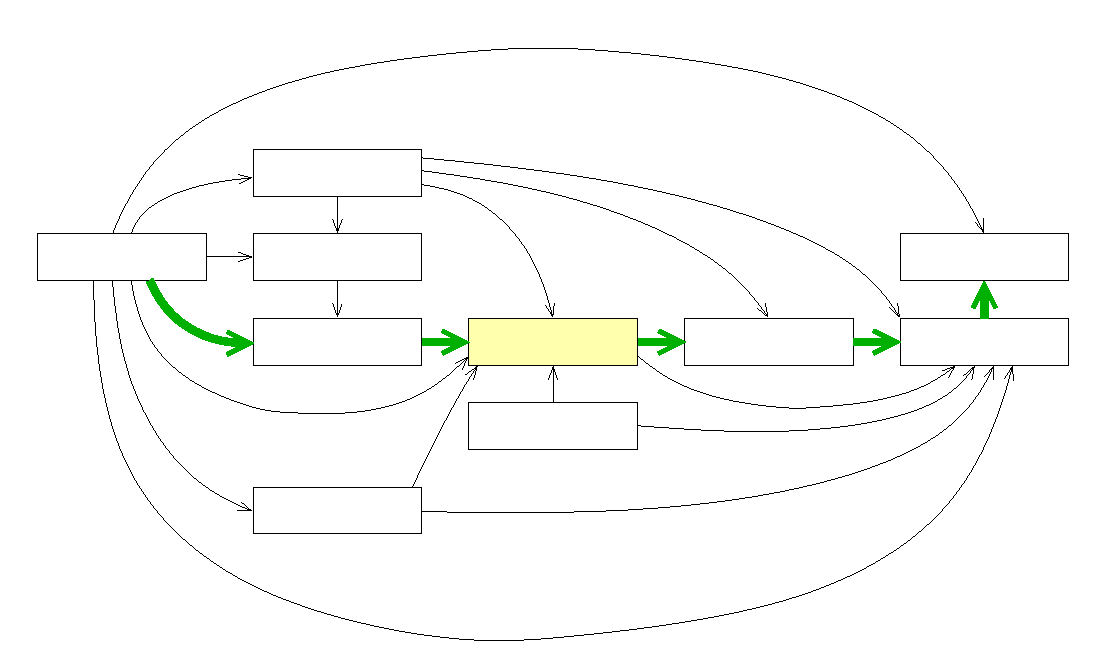
\includegraphics{getdp-struct-formulation}%
\end{picture}%
\setlength{\unitlength}{3947sp}%
%
\begingroup\makeatletter\ifx\SetFigFont\undefined%
\gdef\SetFigFont#1#2#3#4#5{%
  \reset@font\fontsize{#1}{#2pt}%
  \fontfamily{#3}\fontseries{#4}\fontshape{#5}%
  \selectfont}%
\fi\endgroup%
\begin{picture}(8274,4765)(439,-6402)
\put(1126,-3361){\makebox(0,0)[b]{\smash{\SetFigFont{10}{12.0}{\rmdefault}{\mddefault}{\updefault}{\color[rgb]{0,0,0}\code{Group}}%
}}}
\put(2851,-2686){\makebox(0,0)[b]{\smash{\SetFigFont{10}{12.0}{\rmdefault}{\mddefault}{\updefault}{\color[rgb]{0,0,0}\code{Function}}%
}}}
\put(2851,-3361){\makebox(0,0)[b]{\smash{\SetFigFont{10}{12.0}{\rmdefault}{\mddefault}{\updefault}{\color[rgb]{0,0,0}\code{Constraint}}%
}}}
\put(2851,-4036){\makebox(0,0)[b]{\smash{\SetFigFont{10}{12.0}{\rmdefault}{\mddefault}{\updefault}{\color[rgb]{0,0,0}\code{FunctionSpace}}%
}}}
\put(2851,-5386){\makebox(0,0)[b]{\smash{\SetFigFont{10}{12.0}{\rmdefault}{\mddefault}{\updefault}{\color[rgb]{0,0,0}\code{Jacobian}}%
}}}
\put(4576,-4711){\makebox(0,0)[b]{\smash{\SetFigFont{10}{12.0}{\rmdefault}{\mddefault}{\updefault}{\color[rgb]{0,0,0}\code{Integration}}%
}}}
\put(4576,-4036){\makebox(0,0)[b]{\smash{\SetFigFont{10}{12.0}{\rmdefault}{\mddefault}{\updefault}{\color[rgb]{0,0,0}\code{Formulation}}%
}}}
\put(6301,-4036){\makebox(0,0)[b]{\smash{\SetFigFont{10}{12.0}{\rmdefault}{\mddefault}{\updefault}{\color[rgb]{0,0,0}\code{Resolution}}%
}}}
\put(8026,-3361){\makebox(0,0)[b]{\smash{\SetFigFont{10}{12.0}{\rmdefault}{\mddefault}{\updefault}{\color[rgb]{0,0,0}\code{PostOperation}}%
}}}
\put(8026,-4036){\makebox(0,0)[b]{\smash{\SetFigFont{10}{12.0}{\rmdefault}{\mddefault}{\updefault}{\color[rgb]{0,0,0}\code{PostProcessing}}%
}}}
\end{picture}
}}

\chapter{\code{Formulation}: building equations}

\begin{slide}



Example:


\end{slide}

% ---------------------------------------------------------------------------

\background{7\semcm}{4.2\semcm}{\scalebox{0.3}{\begin{picture}(0,0)%
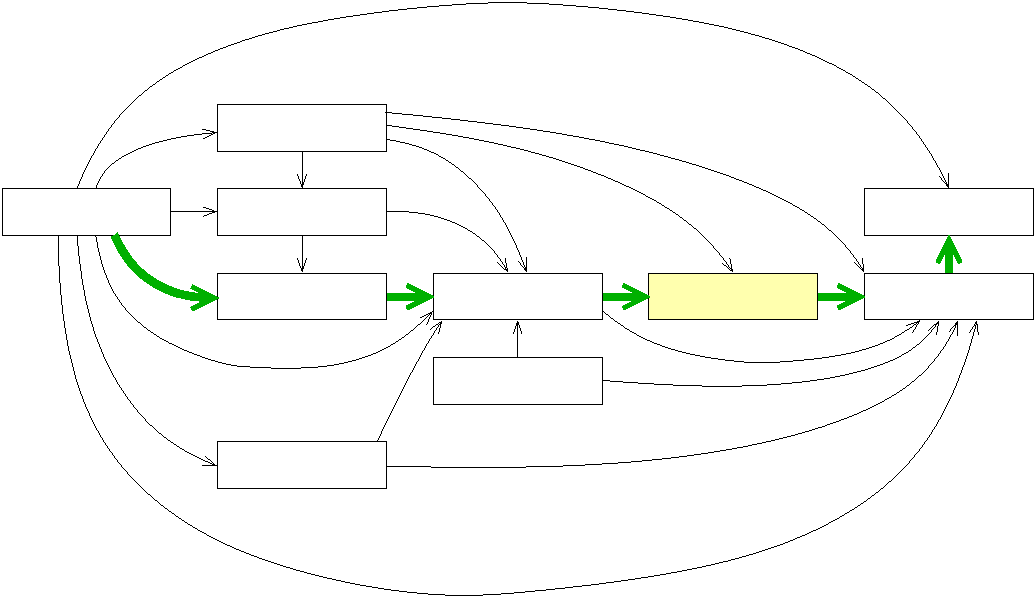
\includegraphics{getdp-struct-resolution}%
\end{picture}%
\setlength{\unitlength}{3947sp}%
%
\begingroup\makeatletter\ifx\SetFigFont\undefined%
\gdef\SetFigFont#1#2#3#4#5{%
  \reset@font\fontsize{#1}{#2pt}%
  \fontfamily{#3}\fontseries{#4}\fontshape{#5}%
  \selectfont}%
\fi\endgroup%
\begin{picture}(8552,4992)(300,-6402)
\put(1126,-3361){\makebox(0,0)[b]{\smash{\SetFigFont{10}{12.0}{\rmdefault}{\mddefault}{\updefault}{\color[rgb]{0,0,0}\code{Group}}%
}}}
\put(2851,-2686){\makebox(0,0)[b]{\smash{\SetFigFont{10}{12.0}{\rmdefault}{\mddefault}{\updefault}{\color[rgb]{0,0,0}\code{Function}}%
}}}
\put(2851,-3361){\makebox(0,0)[b]{\smash{\SetFigFont{10}{12.0}{\rmdefault}{\mddefault}{\updefault}{\color[rgb]{0,0,0}\code{Constraint}}%
}}}
\put(2851,-4036){\makebox(0,0)[b]{\smash{\SetFigFont{10}{12.0}{\rmdefault}{\mddefault}{\updefault}{\color[rgb]{0,0,0}\code{FunctionSpace}}%
}}}
\put(2851,-5386){\makebox(0,0)[b]{\smash{\SetFigFont{10}{12.0}{\rmdefault}{\mddefault}{\updefault}{\color[rgb]{0,0,0}\code{Jacobian}}%
}}}
\put(4576,-4711){\makebox(0,0)[b]{\smash{\SetFigFont{10}{12.0}{\rmdefault}{\mddefault}{\updefault}{\color[rgb]{0,0,0}\code{Integration}}%
}}}
\put(4576,-4036){\makebox(0,0)[b]{\smash{\SetFigFont{10}{12.0}{\rmdefault}{\mddefault}{\updefault}{\color[rgb]{0,0,0}\code{Formulation}}%
}}}
\put(6301,-4036){\makebox(0,0)[b]{\smash{\SetFigFont{10}{12.0}{\rmdefault}{\mddefault}{\updefault}{\color[rgb]{0,0,0}\code{Resolution}}%
}}}
\put(8026,-3361){\makebox(0,0)[b]{\smash{\SetFigFont{10}{12.0}{\rmdefault}{\mddefault}{\updefault}{\color[rgb]{0,0,0}\code{PostOperation}}%
}}}
\put(8026,-4036){\makebox(0,0)[b]{\smash{\SetFigFont{10}{12.0}{\rmdefault}{\mddefault}{\updefault}{\color[rgb]{0,0,0}\code{PostProcessing}}%
}}}
\end{picture}
}}

\chapter{\code{Resolution}: solving systems of equations}

\begin{slide}


Example:


\end{slide}

% ---------------------------------------------------------------------------

\background{7\semcm}{4.2\semcm}{\scalebox{0.3}{\begin{picture}(0,0)%
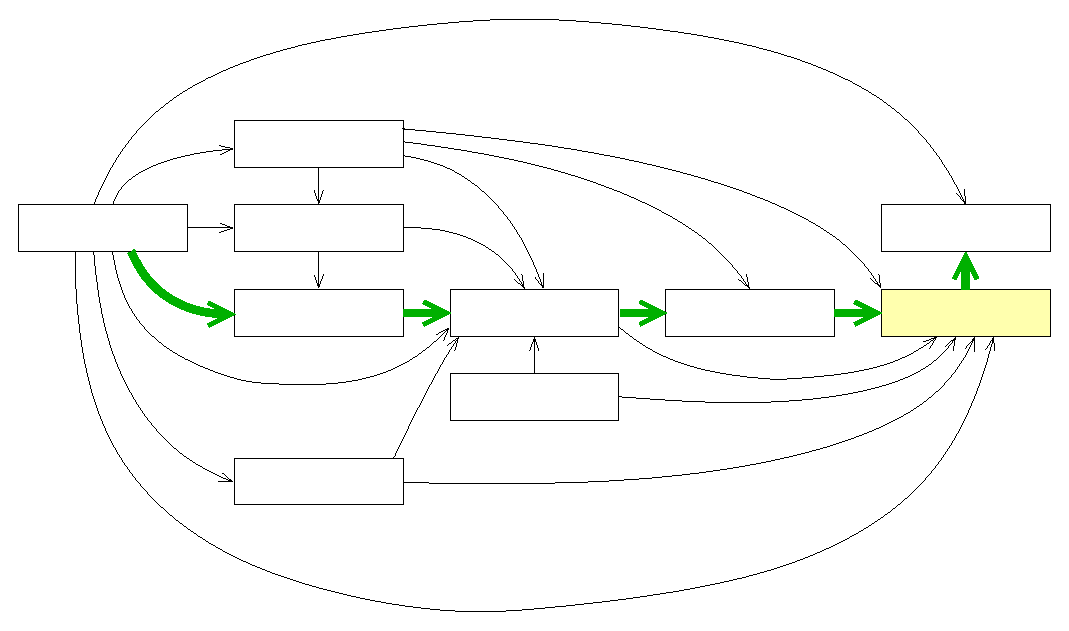
\includegraphics{getdp-struct-postprocessing}%
\end{picture}%
\setlength{\unitlength}{3947sp}%
%
\begingroup\makeatletter\ifx\SetFigFont\undefined%
\gdef\SetFigFont#1#2#3#4#5{%
  \reset@font\fontsize{#1}{#2pt}%
  \fontfamily{#3}\fontseries{#4}\fontshape{#5}%
  \selectfont}%
\fi\endgroup%
\begin{picture}(8274,4765)(439,-6402)
\put(1126,-3361){\makebox(0,0)[b]{\smash{\SetFigFont{10}{12.0}{\rmdefault}{\mddefault}{\updefault}{\color[rgb]{0,0,0}\code{Group}}%
}}}
\put(2851,-2686){\makebox(0,0)[b]{\smash{\SetFigFont{10}{12.0}{\rmdefault}{\mddefault}{\updefault}{\color[rgb]{0,0,0}\code{Function}}%
}}}
\put(2851,-3361){\makebox(0,0)[b]{\smash{\SetFigFont{10}{12.0}{\rmdefault}{\mddefault}{\updefault}{\color[rgb]{0,0,0}\code{Constraint}}%
}}}
\put(2851,-4036){\makebox(0,0)[b]{\smash{\SetFigFont{10}{12.0}{\rmdefault}{\mddefault}{\updefault}{\color[rgb]{0,0,0}\code{FunctionSpace}}%
}}}
\put(2851,-5386){\makebox(0,0)[b]{\smash{\SetFigFont{10}{12.0}{\rmdefault}{\mddefault}{\updefault}{\color[rgb]{0,0,0}\code{Jacobian}}%
}}}
\put(4576,-4711){\makebox(0,0)[b]{\smash{\SetFigFont{10}{12.0}{\rmdefault}{\mddefault}{\updefault}{\color[rgb]{0,0,0}\code{Integration}}%
}}}
\put(4576,-4036){\makebox(0,0)[b]{\smash{\SetFigFont{10}{12.0}{\rmdefault}{\mddefault}{\updefault}{\color[rgb]{0,0,0}\code{Formulation}}%
}}}
\put(6301,-4036){\makebox(0,0)[b]{\smash{\SetFigFont{10}{12.0}{\rmdefault}{\mddefault}{\updefault}{\color[rgb]{0,0,0}\code{Resolution}}%
}}}
\put(8026,-3361){\makebox(0,0)[b]{\smash{\SetFigFont{10}{12.0}{\rmdefault}{\mddefault}{\updefault}{\color[rgb]{0,0,0}\code{PostOperation}}%
}}}
\put(8026,-4036){\makebox(0,0)[b]{\smash{\SetFigFont{10}{12.0}{\rmdefault}{\mddefault}{\updefault}{\color[rgb]{0,0,0}\code{PostProcessing}}%
}}}
\end{picture}
}}

\chapter{\code{PostProcessing}: exploiting computational results}

\begin{slide}



Example:


\end{slide}

% ---------------------------------------------------------------------------

\background{7\semcm}{4.2\semcm}{\scalebox{0.3}{\begin{picture}(0,0)%
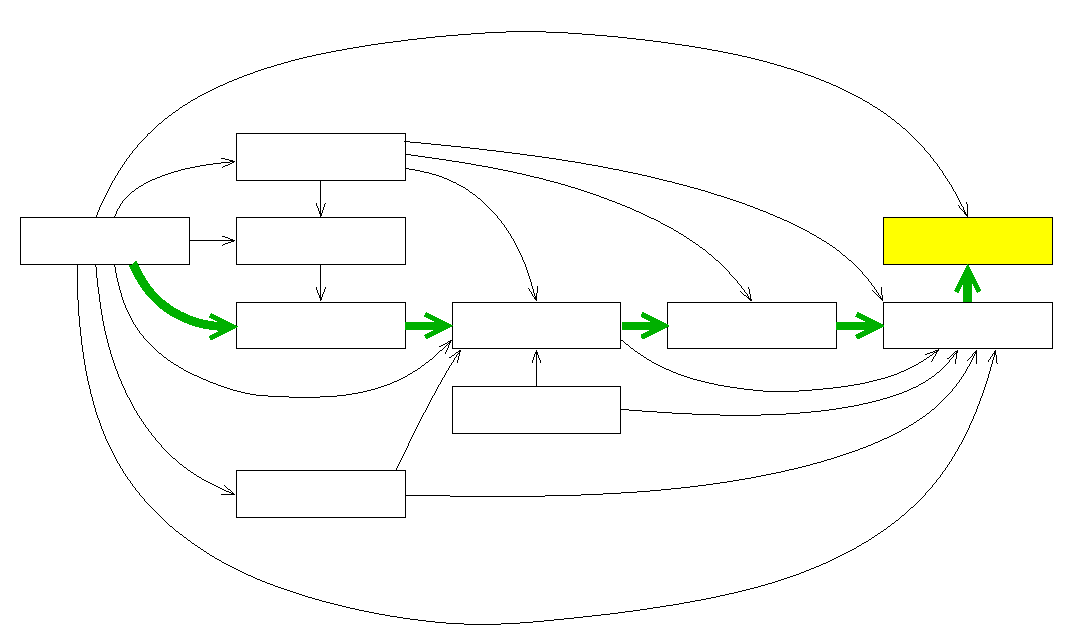
\includegraphics{getdp-struct-postoperation}%
\end{picture}%
\setlength{\unitlength}{3947sp}%
%
\begingroup\makeatletter\ifx\SetFigFont\undefined%
\gdef\SetFigFont#1#2#3#4#5{%
  \reset@font\fontsize{#1}{#2pt}%
  \fontfamily{#3}\fontseries{#4}\fontshape{#5}%
  \selectfont}%
\fi\endgroup%
\begin{picture}(8552,4992)(300,-6402)
\put(1126,-3361){\makebox(0,0)[b]{\smash{\SetFigFont{10}{12.0}{\rmdefault}{\mddefault}{\updefault}{\color[rgb]{0,0,0}\code{Group}}%
}}}
\put(2851,-2686){\makebox(0,0)[b]{\smash{\SetFigFont{10}{12.0}{\rmdefault}{\mddefault}{\updefault}{\color[rgb]{0,0,0}\code{Function}}%
}}}
\put(2851,-3361){\makebox(0,0)[b]{\smash{\SetFigFont{10}{12.0}{\rmdefault}{\mddefault}{\updefault}{\color[rgb]{0,0,0}\code{Constraint}}%
}}}
\put(2851,-4036){\makebox(0,0)[b]{\smash{\SetFigFont{10}{12.0}{\rmdefault}{\mddefault}{\updefault}{\color[rgb]{0,0,0}\code{FunctionSpace}}%
}}}
\put(2851,-5386){\makebox(0,0)[b]{\smash{\SetFigFont{10}{12.0}{\rmdefault}{\mddefault}{\updefault}{\color[rgb]{0,0,0}\code{Jacobian}}%
}}}
\put(4576,-4711){\makebox(0,0)[b]{\smash{\SetFigFont{10}{12.0}{\rmdefault}{\mddefault}{\updefault}{\color[rgb]{0,0,0}\code{Integration}}%
}}}
\put(4576,-4036){\makebox(0,0)[b]{\smash{\SetFigFont{10}{12.0}{\rmdefault}{\mddefault}{\updefault}{\color[rgb]{0,0,0}\code{Formulation}}%
}}}
\put(6301,-4036){\makebox(0,0)[b]{\smash{\SetFigFont{10}{12.0}{\rmdefault}{\mddefault}{\updefault}{\color[rgb]{0,0,0}\code{Resolution}}%
}}}
\put(8026,-3361){\makebox(0,0)[b]{\smash{\SetFigFont{10}{12.0}{\rmdefault}{\mddefault}{\updefault}{\color[rgb]{0,0,0}\code{PostOperation}}%
}}}
\put(8026,-4036){\makebox(0,0)[b]{\smash{\SetFigFont{10}{12.0}{\rmdefault}{\mddefault}{\updefault}{\color[rgb]{0,0,0}\code{PostProcessing}}%
}}}
\end{picture}
}}

\chapter{\code{PostOperation}: exporting results}

\begin{slide}



Example:


\end{slide}

% ---------------------------------------------------------------------------

\background{}{}{}

